\def\Module{Principles of Computer System Design}
\def\Uebung{Exam}
\def\Studentenname{Marco Eilers (dbk726)}
\def\Sub_date{22.01.2013}

\documentclass[12pt,a4paper,fleqn]{article}

\usepackage[utf8]{inputenc}
\usepackage[T1]{fontenc}
\usepackage{fullpage} 
\headsep1cm
\parindent0cm
\usepackage{amssymb, amstext, amsmath}
\usepackage{fancyhdr}
\usepackage{lastpage}
\usepackage{booktabs}
\usepackage{graphicx}
\usepackage{subfigure}
\usepackage{hyperref}
\usepackage{threeparttable}
\usepackage{footnote}
\usepackage{listings}
\usepackage{tikz}
\usepackage[linesnumbered]{algorithm2e}

\makesavenoteenv{tabular}

\usetikzlibrary{arrows,automata}

\lhead{\textbf{\Module}}
\rhead{\Uebung~(Submission: \Sub_date)}

\cfoot{}
\lfoot{\Studentenname}
\rfoot{\thepage\ of \pageref{LastPage}}
\pagestyle{fancy}
\renewcommand{\footrulewidth}{0.4pt}

\newcommand{\code}[1]{{\fontfamily{fvm}\small \selectfont #1}}

%Line spacing between paragraphs
\setlength{\parskip}{6pt}


\begin{document}

\title{\Module\\\Uebung}
\author{\Studentenname}
\maketitle

\section*{Questions} 
\label{sec:questions}

\subsection*{Question 1}
\label{sec:qq1}

\subsubsection*{a)}
\begin{algorithm}[H]


\While{input data left}{
  currentInput = load\_next\_file\_part(inputFile, $B/(k+1)$) \\
  List intermediateResults \\
  \For{(key, value) $\in$ currentInput}{
    result = map(k1, v1) \\
    intermediateResults.add(result) \\
  }
  prefetch\_next\_file\_part(inputFile)\\
  write\_to\_file(intermediateFile, intermediateResults)
  }

\end{algorithm}

The code first loads part of the input file into main memory. $B$ is the number of pages the main memory can hold, and $k$ is the maximal relation between the result of a map call and its input (which I assume exists for every map function), e.g. if a map call may output twice as much data as it gets, $k=2$. This ensures that the input data as well as the resulting intermediate data both fit into memory. Loading more at a time would be desirable, so an optimization might be to drop input pairs as soon as they are evaluated, so that $B/k$ pages could be loaded. \\The algorithm then maps the function on each pair and, as soon as this is done, saves the results back to memory. I assume that we have at least two disks (otherwise we could not use external sorting), which is why we could start prefetching the next part of the input file while we save the intermediate results to disk. The prefetch-call in this function is therefore assumed to be asynchronous and return immediately. \\Here, as well as in the next part, I have assumed that the map and reduce functions actually take some time to calculate, so that it is not possible to just stream the input, apply the map function on the fly, and stream the output to the other disk.

\subsubsection*{b)}

\begin{algorithm}[H]
external\_sort\_by\_key(intermediateFile) \\

\While{intermediate data left}{
  List values \\
  currentInput = load\_next\_file\_part(inputFile, $B - currentMemoryUtil$) \\
  \For{all (key,valueList) $\in$ currentInput that have the same key as the one before}{
    values.addAll(valueList)
  }
  result = reduce(key, values) \\
  
  write\_to\_file(resultFile, result)
}

\end{algorithm}

First we use external sorting to sort the intermediate results by their keys. Then we load the intermediate data bit by bit. Since it is now sorted, we can iterate down the key-value pairs until the key changes, and add all values belonging to the same key to one list, on which we then call the reduce function. Then we save the results. $currentMemoryUtil$ denotes the number of pages of main memory that is \emph{not} used by input we have not yet worked on, i.e. free space and the space occupied by key-value-pairs we have already fed to the reduce function. This means that after every saving operation, we fill the now free memory with as much data from the intermediate data file as we can.

\subsubsection*{c)}
My implementation uses an external sort to group the intermediate results by key, which should have no problem with a skew in the keys. A hash function might simply put all keys into the same bucket if one is unlucky, in which case a second hash function must be applied, which, of course, costs time and necessitates further reading and writing. This cannot happen with a sort based approach. However, my implementation of the reduce phase issues a new read call to disk after every reduce. This is a good solution if all or most keys actually have many values and almost fill out the entire main memory, but it is inefficient if there is a big number of keys with few values. In that case it would be better to read new data from disk only when the input is fully processed. That would make it necessary to delay the call to reduce, keep a list of the current values in memory, and read the next part of the file, each time the end of the currently read input data is reached.

\subsection*{Question 2}
\label{sec:qq2}

\subsubsection*{a)}
\noindent Schedule 1:

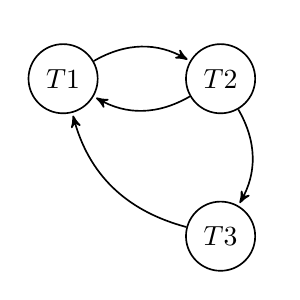
\begin{tikzpicture}[->,>=stealth',shorten >= 1pt,auto,node distance=2.cm,accepting/.style={double distance= 1.5pt},semithick]
\node[state](1) {$T1$};
\node[state] (2) [right of=1] {$T2$};
\node[state] (3) [below of=2] {$T3$};

\path (1) edge [bend left] node {} (2)
      (2) edge [bend left] node {} (3)
          edge [bend left] node {} (1)
      (3) edge [bend left] node {} (1);

\end{tikzpicture}

Schedules are conflict-serializable (i.e. they have an equivalent serial schedule) if and only if there are no cycles in the precedence graph. This is not the case here, since there are actually two cycles in the graph (T1, T2 as well as T1, T2, T3). This means that there cannot be an equivalent serial schedule, since T1 would have to come before T2 (because they read and write X, respectively), T2 has to come before T3 (since they both write Y), but T3 also has to come before T1 (since they both write Y), which is impossible. 

Schedule 2:

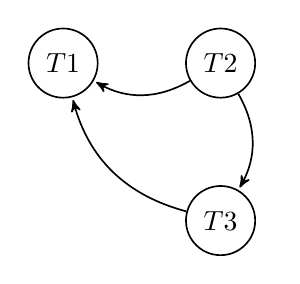
\begin{tikzpicture}[->,>=stealth',shorten >= 1pt,auto,node distance=2.cm,accepting/.style={double distance= 1.5pt},semithick]
\node[state](1) {$T1$};
\node[state] (2) [right of=1] {$T2$};
\node[state] (3) [below of=2] {$T3$};

\path (2) edge [bend left] node {} (3)
          edge [bend left] node {} (1)
      (3) edge [bend left] node {} (1);

\end{tikzpicture}

There are no cycles in this graph, which means that this schedule is conflict-serializable. An equivalent serial schedule would be T2 $\rightarrow$ T3 $\rightarrow$ T1.


\subsubsection*{b)}
Schedule 1 could not have been generated by a scheduler using Strict 2PL. First of all, Strict 2PL allows only conflict-serializable schedules (see \cite{Ramakrishnan2003}), so the fact that this schedule is not conflict-serializable rules out that Strict 2PL generated it. In Strict 2PL, resources are locked when needed by a transaction, and the locks are only released when the transaction is completed, meaning that all of a transaction's locks are released at once at its end. In schedule 1, T1 would acquire a shared (read) lock on X at the beginning. But right after that, T2 needs an exclusive (write) lock on X. Since T1 has not yet committed and T2 cannot get an exclusive lock while another transaction holds a shared lock on the same resource, this is impossible. There are other conflicts as well: T2 needs a write lock on Y in its second step, but after that T3 and subsequently T1 also write Y, although T2 has not yet committed and still holds the lock.

Schedule 2, on the other hand, \emph{could} be the product of a Strict 2PL scheduler. The following shows the transaction schedule including lock operations where S(X) means that a shared (read) lock is acquired for X, and X(Y) means that an exclusive lock is acquired for Y. Unlocking is implicit: all locks are released when a transaction commits.

\begin{align*}
  \text{T1: } & \text{S(X)} & \text{R(X)} & & & & & & & & & \text{X(Y)} & \text{W(Y) } & \text{C} \\
  \text{T2: } & & & \text{X(Y)} & \text{W(Y) } & \text{X(Z)} & \text{W(Z) } & \text{C} & & & & & & \\
  \text{T3: } & & & & & & & & \text{X(Y) } & \text{W(Y)} & \text{C} & & & 
\end{align*} 

\subsection*{Question 3}
\label{sec:qq3}

\subsubsection*{a)}
\begin{enumerate}
  \item See table \ref{tab:transactions} for the transaction table and table \ref{tab:dirty} for the dirty page table after the analysis phase. The status U indicates that a transaction has to be undone.
  \item The set of loser transactions is $\{T1, T2\}$, the set of winner transactions is $\{T3\}$.
  \item The redo phase starts at LSN 3. The undo phase ends at LSN 3.
  \item The set of log records that may cause changes to be rewritten during the redo phase is $\{3,4,5,6,7,8,11\}$.
  \item The set of log records undone during the undo phase is $\{5,4,3\}$. LSN 11 is also evaluated by the UNDO algorithm, but is not actually undone, since it is already a CLR.
  \item See table \ref{tab:after} for the contents of the log after the recovery procedure.
\end{enumerate}

\begin{table}
  \centering
  \begin{tabular}{c | c | c}
  Transaction ID & Status & lastLSN \\ \hline
  T1 & U & 3\\
  T2 & U & 11
  \end{tabular}
  \caption{Transaction table after the analysis phase}
  \label{tab:transactions}
\end{table}

\begin{table}
  \centering
  \begin{tabular}{c|c}
  Page & recLSN \\ \hline
  P1 & 3 \\
  P7 & 5 \\
  P3 & 6 \\
  P5 & 8 
  \end{tabular}
  \caption{Dirty page table after the analysis phase}
  \label{tab:dirty}
\end{table}

\begin{table}
  \centering
  \begin{tabular}{l | l | l | l | l | l}
  LSN & LAST\_LSN & TRAN\_ID & TYPE & PAGE\_ID  & UNDONEXTLSN \\ \hline
  1 & - & - & begin CKPT & - & -\\
  2 & - & - & end CKPT & - & -\\
  3 & NULL & T1 & update & P1 & -\\
  4 & NULL & T2 & update & P1 & -\\
  5 & 4 & T2 & update & P7 & -\\
  6 & NULL & T3 & update & P3 & -\\
  7 & 5 & T2 & update & P3 & -\\
  8 & 6 & T3 & update & P5 & -\\
  9 & 8 & T3 & commit & - & -\\
  10 & 7 & T2 & abort & - & -\\
  11 & 10 & T2 & CLR & P3 & 5 \\
  12 & 9 & T3 & end & - & - \\
  13 & 11 & T2 & CLR & P7 & 4 \\
  14 & 13 & T2 & CLR & P1 & NULL \\
  15 & 14 & T2 & end & - & - \\
  16 & 3 & T1 & CLR & P1 & NULL \\
  17 & 16 & T1 & end & - & -
    
  \end{tabular}
  \caption{The log after the recovery procedure completes}
  \label{tab:after}
\end{table}

\subsubsection*{b)}
The LSN where the redo phase \emph{starts} is the smallest recLSN value in the dirty page table. Since the dirty page table contains the pages for which changes might not have been stored on stable (or at least permanent) storage yet, this is the earliest action whose changes might not have been written to disk yet. Since ARIES does not force all dirty pages to disk even when creating a checkpoint, this action might possibly be very far up in the log.

The LSN where the undo phase \emph{ends} is the first LSN of the loser transaction that started first, i.e. the first LSN of the oldest transaction that did not commit before the crash, or that aborted but was not completely rolled back before the crash.  This can also potentially be quite far up in the log, if a very long running transaction that was close to being committed has to be rolled back because of the crash.

\section*{Programming Task} 
\label{sec:programming}

\subsection*{Question 1}
\label{sec:pq1}

I used a simple hash function to decide which branch is stored on which partition. Since branch identifiers are integers, I simply take the branch identifier modulo the number of existing branches. The advantages of this approach are the following:
\begin{itemize}
  \item It is computationally efficient, since only a simple arithmetic operation has to be carried out.
  \item It will lead to the same result in all proxies (provided that the same hash value is assigned to the same partition in all proxies, which I make sure they are).
  \item It does not require the proxy to create an additional data structure to keep track of the assignments, as a round robin algorithm would.
  \item In comparison to a distribution by range, this hash may be less prone to skewed data (e.g. most accounts being within a specific range of numbers) and, more importantly, it results in a more easily extendable product: If new branches are added, a hash like this can incorporate them without problems, whereas a range-based system might have to be adjusted if the range of used branch identifiers gets bigger.
\end{itemize}
Downsides of this approach are that it is impossible to add new partitions at runtime and necessitates a redistribution of branches in case a new partition is added offline (but this was not required for our solution), and that the distribution of accounts over the branches is not considered, so that accounts might be distributed very unevenly over the partitions if their number varies strongly between branches. As with all hash functions, it is, of course, possible (but not likely) that one has bad luck and all or most branches are assigned to one partition. We do not have to worry about an adversary choosing branch IDs in order for our distribution to fail, since I assume banks choose their branch identifiers themselves.
Therefore I do not make any assumptions about the distribution of branches (e.g. they do not have to be continuous) except that schemes like only using every second ID are not used.

I chose JAX-WS as my RPC mechanism. I prefer Java over C\# as a programming language, so WCF was not an option for me. Compared to Java's RMI, I preferred JAX-WS because it is platform independent and can be used by all kinds of clients, which do not necessarily need to be based on Java. RMI, on the other hand, transmits serialized Java objects, and is therefore quite platform dependent. While RMI probably has a more efficient way of transmitting data (SOAP, which is XML-based, is not the most efficient way of storing data), our application only requires us to transmit a small number of integers and doubles in each request, so efficient data representation is not really an issue here. In contrast to other methods of exposing web services, JAX-WS is comparatively transparent to the programmer, since remote procedure calls are simply function calls in the code, which makes programming a lot easier. JAX-WS seems to have less than optimal scalability on the client side, as several internet articles indicate (see for example \cite{Pollmeier2011}), which might haunt me in the experiment, but since this only marginally affects the server side, it is still reasonable to implement the service using JAX-WS.

In general, I tried to use a modular design in my application whereever possible. An example for this is the distribution of branches over partitions: Since my partitions are completely ignorant of the outside world and initialization files do not contain any distribution information, the distribution algorithm can easily be exchanged by simply using a different class implementing the \texttt{Partitioner} interface in the proxy. Another example is the implementation of branches, for which I implemented two versions with different concurrency control (see the following question) which can also easily be exchanged.

\subsection*{Question 2}
\label{sec:pq2}
I ensured atomicity of the AccountManager's operations by using locks on the account level. For every account there is one instance of Java's ReentrantReadWriteLock, which is locked whenever a given account is read or written to. I use conservative strict 2PL; I always know at the beginning of an operation which accounts have to be locked, and since the service's basic operations are mostly quite simple, postponing the locking until right before the account is accessed would not lead to a big performance gain. Most operations lock the necessary accounts for write access, only \texttt{calculateExposure} uses a shared (read) lock. In order to avoid deadlocks, all accounts are always locked in the order of their IDs from lowest to highest. Only methods that are exposed to the client use locks; the only other major method, \texttt{setBalance}, is used to create an account during initialization and is only called once. Since partitions are only available to the client \emph{after} they have been initialized, this operation never runs alongside other methods and therefore needs no locks. The locking mechanism is implemented at the branch level, i.e. every branch has a table of locks for its accounts. Since I was curious about the difference in performance, I also implemented a branch using an optimistic approach (the Kung-Robinson Model), but I will use this solely in the experiment and only defend the locking approach in the following questions.

Conservative Strict 2PL allows only serializable schedules, i.e. schedules which are equivalent to at least one serial schedule. This could also be achieved by using a single global lock which makes sure that only one transaction runs at a time. It is easy to see why Conservative Strict 2PL and a global lock are logically equivalent: Conservative Strict 2PL locks all accounts which are used by an operation for the entire duration of said operation. Any other operation which also uses at least one of these accounts must therefore be executed either before or after this operation. The same is true with a global lock. However, operations which only affect other accounts do not affect this operation at all (and can therefore run concurrently), which means that in a serial schedule (which would be enforced by a global lock), those transactions could be scheduled either before or after this transaction, and the result would be the same.  \\
As stated before, I always lock accounts in the order of their ID. It is just as easy to see why this prevents deadlocks: Any two operations which both need access to accounts $A$ and $B$ will try to lock the account with the lower ID first, and only one of them will succeed. Therefore it is impossible that one thread has a lock on $B$ and waits for $A$ while another thread has $A$ but waits for $B$.

For an estimate of how much throughput a service like AccountManager would actually need, I have tried to find statistics for big European banks. I could only find actual numbers for Nordea Bank on Wikipedia (see \cite{Wikipedia}), which are only partly backed by more credible sources, but they should be accurate enough for a quick sketch. Nordea's 5.9 million online customers carry out 290 million online payments per year. The bank has 11 million private and 700,000 corporate customers and 1,400 branches. If we assume that each customer has three accounts, and that corporate customers carry out ten times as many payments as private ones (I do not know if this is even remotely true, but I think it is reasonable to assume that corporate customers carry out more transfers than private ones), this results in 3.51 million accounts  and $290 \times \frac{11}{5.9} + 290 \times \frac{10 \times 0.7}{5.9} \approx  885$ million payments per year, which means 250 transfers per account per year, and altogether 28 transfers per second. Even if we assume that all payments are made during business hours (eight hours a day, five days a week), we have only about 117 requests per second. Considering that these payments will be carried out on different accounts, it seems very unlikely that there would often be two requests for the same account at the same time. 
Nevertheless, our service should also be able to deal with "rush hours", and we want it to scale well in case our organization grows further, which is why it should definitely be possible to concurrently carry out several requests on the same branch. A queueing mechanism, while very easy to implement, would therefore not be my my first choice. 
At first glance, this seems to be a perfect fit for optimistic concurrency control, since the low number of expected conflicts means that the overhead of locking could be avoided for most transactions. However, I decided to use a lock-based approach for the following reasons:
\begin{itemize}
  \item All but one of our operations are write operations. Optimistic concurrency control is more suitable for systems with many read-only operations, since they do not conflict with others.
  \item The very short duration of single requests (due to their simplicity) means locking has less overhead than in other scenarios, since the access to resources will almost never be blocked for a long time.
  \item The optimistic algorithm has itself certain overheads: Transactions have to be kept in memory after they are done, and the verification phase is again carried out by only a single thread. 
  \item Java's ReadWriteLocks are quite efficiently implemented, whereas I am not sure how well my own (necessarily much less optimized) implementation of optimistic CC would perform.
  \item The \texttt{calculateExposure} operation accesses all accounts, and will therefore \emph{always} be redone in an optimistic model when any (write) transaction on the same branch occurs concurrently. This makes the service's performance much less predictable.
\end{itemize}
I still implemented a branch using an optimistic approach for comparison, since it seems like a reasonably good fit in theory; see question 4 for the actual differences in performance.

\subsection*{Question 3}
\label{sec:pq3}
In general, I used a combination of manual and automated tests on my service. All automated tests were implemented using JUnit. I wrote some whitebox tests that check basic functionality of single classes, but mostly performed blackbox tests that utilize the proxy's interface just like an actual client would. 

I have written two main tests which try to make sure that all operations are atomic, both of which can be found in the class \texttt{AtomicTest}. \texttt{transferExposureAtomicity} lets ten client threads transfer money between six accounts of the same branch in parallel. At the same time, four threads request the branch's exposure again and again. All of the accounts are initialized to have highly negative balances, which is why they all contribute to the calculated exposure. A transfer of a small amount from one of these accounts to another can never change the overall exposure, since the money that is credited to one account is debited from another. If, however, either \texttt{calculateExposure} or \texttt{transfer} are not atomic, it would be possible (and, given enough iterations, likely) that an exposure-calculating thread visits one account involved in a transfer \emph{before} the transfer has been applied to it, and the other account \emph{after} the transfer has been applied, thus resulting in a change of the overall exposure. This test therefore executes 200 transfers per thread and asserts that the exposure always remains the same. \\The second automated test lets eight threads perform various write-transactions (credit, debit and transfer) in parallel on the same branch and saves records of all those transactions. Afterwards, it calculates the expected exposure based on the recorded transactions, and makes sure that \texttt{calculateExposure} returns the same value. If one of the write transactions was not atomic, the result would very likely not be identical, since there would probably be read-write conflicts. For example, when two threads want to credit money to one account, the first thread could first read the current value, then the second thread could read the same value, the first thread could write an updated value, and the second thread could overwrite this value with its own result, which would no longer reflect the change made by the first thread. \\Apart from that, I performed some manual tests, like putting a \texttt{Thread.sleep} statement in the \texttt{calculateExposure} method in order to slow it sown, and making sure that parallel write requests return only after the exposure has been returned.

In order to test the system's error handling, I wrote two additional automated tests. The first one, \texttt{exceptionTest}, calls the service's methods with various kinds of invalid inputs, and makes sure that (only) the appropriate exceptions are thrown. \texttt{failSoftTest}, on the other hand, assumes that several partitions are available and that at least one of them is running on a separate Tomcat instance. It first runs a few operations on different branches to make sure all branches are actually accessible. Then it shuts down the second Tomcat instance, and makes sure that subsequent request concerning branches on that partition fail with an \texttt{InexistentBranchException}, whereas requests concerning branches on the other partition still run correctly. I also performed several manual tests, like shutting down single partitions via Tomcat's manager interface and checking if requests concerning branches on other partitions still work, or shutting down \emph{all} partitions, and making sure that the proxy responds to all subsequent requests by raising an \texttt{InexistentBranchException}.

\subsection*{Question 4}
\label{sec:pq4}

For my experiment, I used the three (virtual) servers described in table \ref{tab:setup}, all of which are hosted on Microsoft Azure in the same region (Southeast Asia). All web services were hosted on an Apache Tomcat, version 7.0.35. The client which uses the service and measures the time, as well as a proxy service, were run on Kaninbyen, which is the strongest of the three servers, in an effort to keep hardware limitations on the client side from interfering with the measurements. I hosted a total of one to four partitions, equally distributed if possible, on Kaninchenstadt and Bunnytown. Originally, I intended to use a higher number of partitions, but it turned out that four partitions were already more than enough to completely utilize the available hardware. \\My test client (see the class \texttt{Experiment}) starts several threads, each of which performs 1000 requests on the service, equally distributed between the four available methods. I assumed that the workload for different branches and accounts is skewed: Within a branch, 20 percent of the accounts will receive 80 percent of the requests (according to the 80-20 rule often used in economics; for the distribution function see the self-similar function in \cite{Gray1994}). I also assumed that the workload on branches is still skewed, but to a lesser degree (since there would hardly be entire branches with almost no work), which is why I used a self-similar distribution where 30 percent of branches get 70 percent of the requests. For every number of partitions, I tried which number of client threads generates the highest total throughput (trying each number three times and keeping the attempt with the highest throughput). For every run, I measured the time between the start of the first client thread and the moment all client threads had terminated, i.e. the total time it took the service to process all requests, and stored the total number of requests divided by this time (i.e. the throughput). Since Java uses Just-In-Time compilation, I always ran the experiment several times before storing the results, so that the JRE has enough time to optimize the bytecode. \\
Each partition had 100 branches consisting of 5000 accounts on average (the specific numbers were taken from a gaussian distribution with mean 5000 and standard deviation 2000), which means that the size of the overall data set grew linearly with the addition of more partitions.
\\For the case of only one partition, I ran the experiment with both the locking based and the optimistic currency control branch.

First of all, the results show that my decision to use locking over optimistic concurrency control turned out to be right, at least for the conditions of this experiment (which, of course, do not reflect actual usage conditions). See figure \ref{fig:1par} for a comparison of both concurrency control versions: while the difference is not big, locking is slightly faster in all cases. The figure also shows that one partition could handle a maximum of 1115 requests per second, using 13 client threads. Figure \ref{fig:throughput} shows the maximum throughput for different numbers of partitions. With each additional partition, the throughput is higher than before, but the increase is only really noticable for two partitions compared to one. With two partitions, there is a maximum throughput of 1637 requests per second, or a speedup of 1.47; with four partitions, the speedup is 1.54. I did not run the experiment with higher numbers of partitions, because at this point, hardware limitations prevented any further speedup worth mentioning. In fact, even with only two partitions (where the maximal throughput was reached with 14 client threads), the server hosting the client and proxy was already running near 100 percent utilization, which is why I suspect that the speedup would have been higher (and closer to 2) if not for the limited speed of client and proxy. The limited scalability of JAX-WS clients, as discussed above, may also play a role here. \\So we observe that the service's throughput does scale, though not perfectly, with the addition of more partitions, although it would probably have done better if additional hardware was added for each partition as well, and more proxies and physical clients might have improved the scalability even more. We also notice that adding new partitions even without new hardware still improves the throughput slightly, which may be because the additional branches and accounts mean a better distribution of requests over all branches and thus fewer conflicts. In any case, the addition of more accounts and branches does not seem to hurt the performance.

\begin{table}
\begin{tabular}{|l|l|l|l|}
\hline 
Server & Kaninbyen & Kaninchenstadt & Bunnytown \\ 
\hline 
CPU & 4 $\times$ 1.6GHz, 64 bit & 2 $\times$ 1.6GHz, 64 bit &  2 $\times$ 1.6GHz, 64 bit \\
\hline
RAM & 7 GB & 3.5 GB & 3.5 GB \\
\hline
OS & Ubuntu Server 12.04.1 & Windows Server 2012 & Ubuntu Server 12.04.1 \\
\hline 
JRE & OpenJDK 1.7.0\_09 & Oracle JRE 1.7.0\_11 & OpenJDK 1.7.0\_09 \\
\hline
\end{tabular} 
\caption{Servers used for the experiment}
\label{tab:setup}
\end{table}

\begin{figure}
\centering
  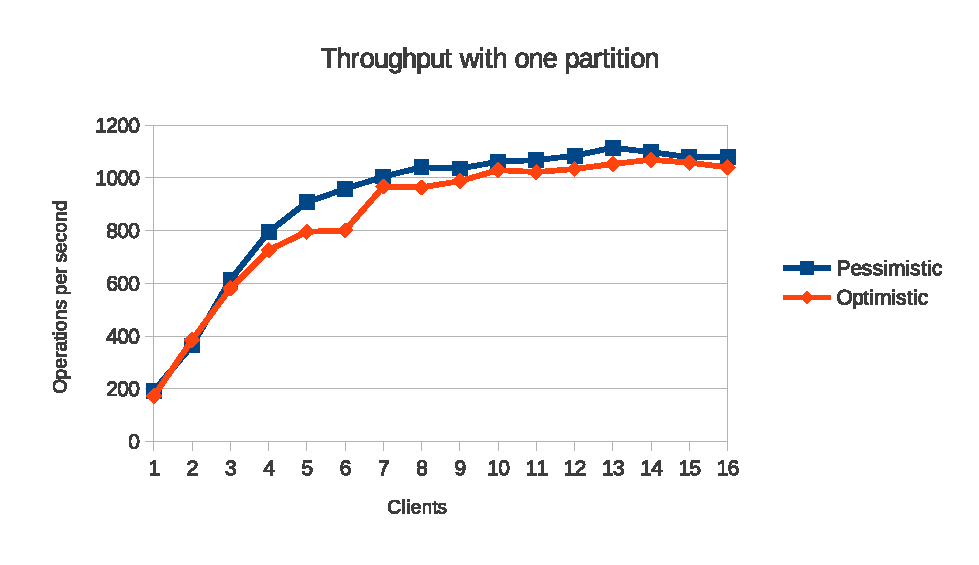
\includegraphics[width=0.8\textwidth]{1par}\\
  \caption{Throughput of one partition with different implementations of concurrency control}
  \label{fig:1par}
\end{figure}

\begin{figure}
\centering
  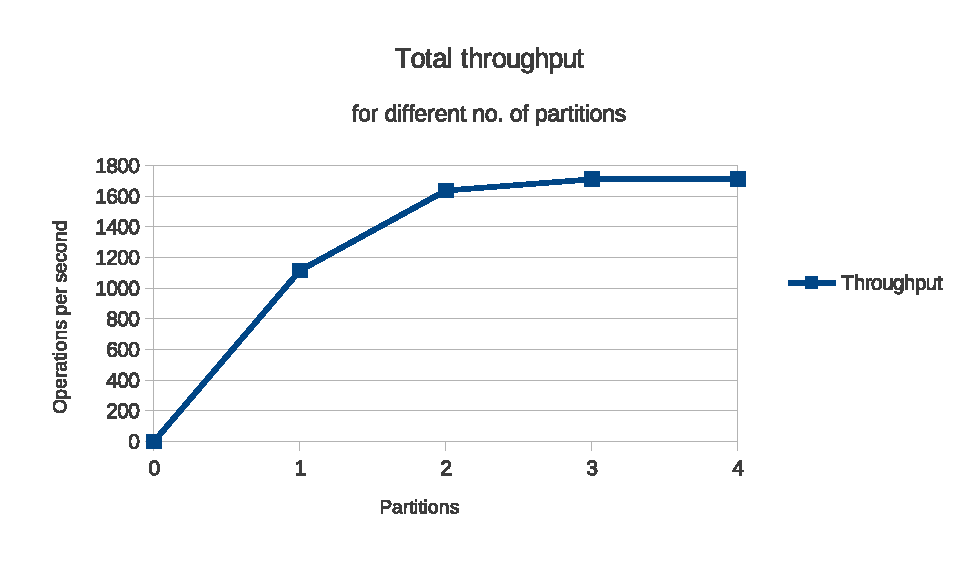
\includegraphics[width=0.8\textwidth]{throughput}\\
  \caption{Throughput for different numbers of partitions}
  \label{fig:throughput}
\end{figure}


\begin{thebibliography}{1}

\bibitem[Gray1994]{Gray1994} Gray et al.: Quickly Generating Billion-Record Synthetic Databases. SIGMOD 1994: 243 - 252. Tech report available at: \url{http://research.microsoft.com/~gray/papers/SyntheticDataGen.doc}.

\bibitem[Wikipedia]{Wikipedia} Wikipedia, the free encyclopedia: Nordea Bank. Retrieved from: \url{http://en.wikipedia.org/wiki/Nordea_Bank}.

\bibitem[Ramakrishnan2003]{Ramakrishnan2003} R. Ramakrishnan \& J. Gehrke: Database Management Systems. Third Edition. McGraw-Hill, 2003, as found in: Principles of Computer System Design - DIKU Course Compendium. DIKU 2012.

\bibitem[Pollmeier2011]{Pollmeier2011} M. Pollmeier: Performance testing with insights into JaxWS client scalability. May 2011. Retrieved from: \url{http://www.michaelpollmeier.com/performance-testing-with-insights-into-jaxws-client-scalability/}.


\end{thebibliography}



\end{document}
